\documentclass[border=3pt]{standalone}
\usepackage{fontspec,amsmath,amssymb,newtxmath,bm,tikz}
\setmainfont{TeX Gyre Termes}
\usetikzlibrary{arrows.meta,positioning,calc}
\newcommand{\E}{\mathbb E}
\newcommand{\TV}{\operatorname{TV}}
\begin{document}
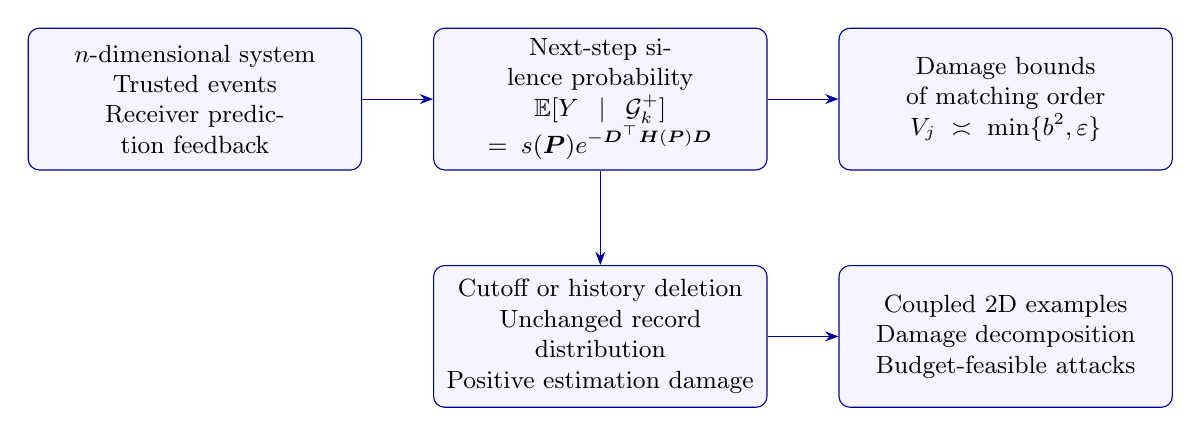
\begin{tikzpicture}[>=Stealth,font=\fontsize{9}{11}\selectfont,
 box/.style={draw=blue!60!black,fill=blue!4,rounded corners,align=center,minimum height=18mm,text width=40mm},edge/.style={->,draw=blue!60!black}]
\node[box] (a) {$n$-dimensional system\\Trusted events\\Receiver prediction feedback};
\node[box,right=9mm of a] (b) {Next-step silence probability\\$\E[Y\mid\mathcal G_k^+]$\\$=s({\bm{P}})e^{-{\bm{D}}^\top {\bm{H}}({\bm{P}}){\bm{D}}}$};
\node[box,right=9mm of b] (c) {Damage bounds of matching order\\$V_j\asymp\min\{b^2,\varepsilon\}$};
\node[box,below=12mm of b] (d) {Cutoff or history deletion\\Unchanged record distribution\\Positive estimation damage};
\node[box,below=12mm of c] (e) {Coupled 2D examples\\Damage decomposition\\Budget-feasible attacks};
\draw[edge] (a)--(b);\draw[edge] (b)--(c);\draw[edge] (b)--(d);\draw[edge] (d)--(e);
\end{tikzpicture}
\end{document}
